\section{Ваши фамилия, имя, отчество, номер группы.}

\begin{itemize}
  \item \normalsize{{Державин Андрей Андреевич, группа Б01-901}}
  \item \normalsize{{Хайдар\'{и} Фарид Гулович, группа Б01-901}}
  \item \normalsize{{Шурыгин Антон Алексеевич, группа Б01-909}}
  \item \normalsize{{Лирисм\'{а}н Карина Сергеевна, группа Б03-001}}
\end{itemize}

\section{Фамилия, имя, отчество лектора.} 

Донов Геннадий Иннокентьевич.

\section{Чем отличается микроконтроллер от микропроцессора.}

Микропроцессор -- вычислительное ядро без переферии. В то время как микроконтроллер 
помимо ядра включает в себя таймеры, порты ввода-вывода, АЦП.

\section{Какие тактовые частоты могут быть у ATmega8535.}
1, 2, 4 МГц от внутреннего генератора.
0.1 - 16 МГц от внешнего генератора.

\section{Какие таймеры есть у ATmega8535.}
У ATmega8535 есть следующие таймеры:
\begin{itemize}
  \item два $8$-разрядных таймера
  \item один $16$-разрядный таймер
\end{itemize}

\section{Внутренняя структура МК.}
Многие современные МК имеют структуру, приведённую на рис. \ref{img::1_2_1}.
Отмеченные на рисунке блоки, входящие в состав микроконтроллера,
выполняют следующие функции:
\begin{figure}[h]
  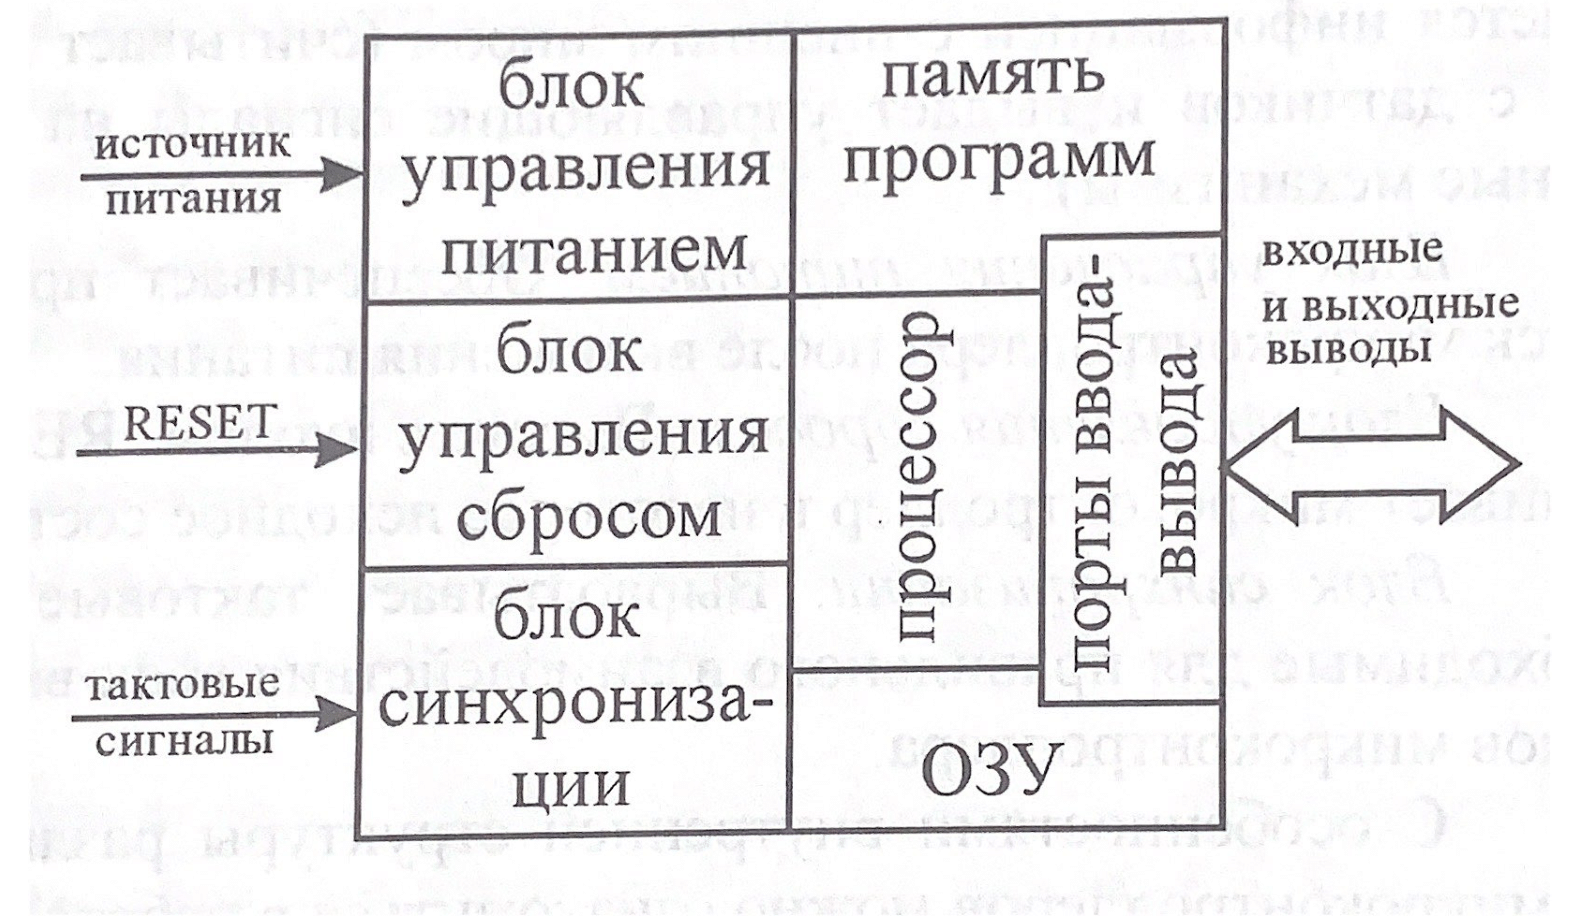
\includegraphics[width=\linewidth]{./src/pics/1.2.1.png}
  \caption{Внутрення структура микроконтроллера.}
  \label{img::1_2_1}
\end{figure}

\begin{itemize}
  \item \textit{Процессор}\\
  Обеспечение обработки информации путём выполнения команды в соответствии 
  с системой команд микроконтроллера.
  \item \textit{Память программ}\\
  Хранение программы, в соответствии с которой работает микроконтроллер.
  \item \textit{ОЗУ}\\
  Другое название ~---~ \textbf{RAM} (Random Access Memory).
  Хранение промежуточных результатов.
  \item \textit{Порты ввода/вывода}\\
  Осуществление обмена информацией с внешним миром.
  \item \textit{Блок управления питанием}\\
  Обеспечение правильности запуска микроконтроллера
  после включения питания.
  \item \textit{Блок управления сбросом}\\
  Установка вместе с входом $RESET$ микроконтроллера в 
  некоторое исходное состояние.
  \item \textit{Блок синхронизации}\\
  Выработка тактовых сигналов, необходимых для правильного взаимодействия 
  всех внутренних блоков микроконтроллера.
\end{itemize}

\section{Какие значения записаны в TCCR после сигнала RESET.}
После сигнала $RESET$ все разряды будут установлены в нулевое значение.

\section{Порт А. Сколько прерываний и сколько регистров ввода/вывода принадлежит порту А. Назначение этих регистров ввода/вывода.}

Для порта А не предназначено ни одного прерывания. Три регистра: PORTA, DDRA, PINA.
DDRn - на вход или выход работает вывод, PORTn - выходное значение, PINn - входное значение.


\section{Регистр SREG. Назначение его  разрядов.}
Регистр $SREG$ ~---~ $8$-разрядный регистр признаков (регистр флагов).
Назначение разрядов приведено на рис. \ref{img::2_3_2}
\begin{figure}[h]
  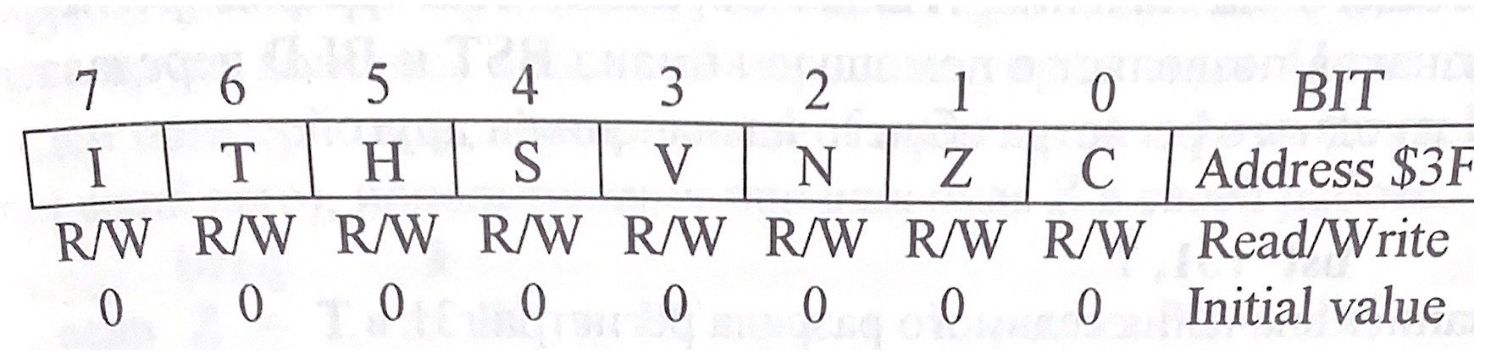
\includegraphics[width=\linewidth]{./src/pics/2.3.2.png}
  \caption{Назначение разрядов регистра $SREG$}
  \label{img::2_3_2}
\end{figure}
Рассмотрим подробнее назначение разрядов:
\begin{itemize}
  \item Бит $7$ -- $I$\\
  Глобальное разрешение прерываний.
  Если в этом разряде нуль, то никакие прерывания не будут обрабатываться.
  Бит обнуляется при возникновении любого прерывания, 
  и автоматически выставляется в единицу при выходе из прерывания.
  \item Бит $6$ -- $T$\\
  Временное хранение бита.
  С помощью команд $BST$ и $BLD$ позволяет передавать
  бит из одного регистра общего назначения в другой. Например,
  следующий код:
  \begin{verbatim}
    bst r31, 7 ; запись значения седьмого разряда регистра r31 в T
    bld r0, 3  ; запись из T в третий разряд регистра r0
  \end{verbatim}
  \item Бит $5$ -- $H$\\
  Признак переноса между полубайтами.
  \item Бит $4$ -- $S$\\
  Равен сумме по модулю $2$ содержимого третьего и второго разряда
  регистра $SREG$.
  \item Бит $3$ -- $V$\\
  Признак переполнения.
  \item Бит $2$ -- $N$\\
  Признак отрицательного результата.
  \item Бит $1$ -- $Z$\\
  Признак нуля.
  \item Бит $0$ -- $C$\\
  Признак переноса.
\end{itemize}

\section{Почему после сигнала RESET все прерывания запрещены.}
Для обеспечения корректной инициализации работы
микроконтроллера.

\section{Приведите пример использования разряда Т в регистре SREG.}
\begin{verbatim}
  bst r30, 5 ; запись значения пятого разряда регистра r30 в T
\end{verbatim}


\section{Таймер 0. Режимы работы, количество прерываний, регистры ввода/вывода, принадлежащие таймеру 0.}

Режимы работы:
\begin{itemize}
  \item Normal (0)\\
  Счётчик $TCNT0$ функционирует как обычный суммирующий счётчик.
  \item PWM Phase Correct (1)\\
  Режим ШИМ с точной фазой. Предназначен для генерации сигналов с 
  широтно-импульсной модуляцией.
  \item CTC -- Clear Timer on Compare match (2)\\
  Режим счёта по модулю, который определяется содержимым регистра $OCR0$.
  \item Fast PWM (3) \\
  Быстродействующий ШИМ. Позволяет генерировать высокочастотный сигнал 
  с широтно-импульсной модуляцией.
\end{itemize}

Прерывания:
\begin{itemize}
  \item $TIMER0\_OVF$ -- переполнение таймера
  \item $TIMER0\_COMP$ -- содержимое счётчика $TCNT0$ совпадает с 
  содержимым регистра $OCR0$.
\end{itemize}

Имеет $3$ регистра ввода-вывода. Ещё $2$ регистра используются совместно 
с таймерами $1$ и $2$:
\begin{itemize}
  \item $TCCR0$ -- Регистр контроля
  \item $SFIOR$ -- Регистр обнуления
  \item $TIMSK$ -- Регистр прерывания
  \item $TIFR$ -- Регистр флагов прерываний
\end{itemize}

Также есть возможность использования двух выводов микроконтроллера:
\begin{itemize}
  \item вход $T0$ ~---~ Timer/Counter0 External Counter Input -- вывод $PB0$
  \item выход $OC0$ ~---~ Timer/Counter0 Output Compare Match Output -- вывод $PB3$
\end{itemize}

\section{В каких режимах таймера 0 порог изменяется не сразу (двойная буферизация записи) при записи нового значения в регистр порога с помощью команды OUT. }
\begin{itemize}
  \item PWM Phase Correct (1)\\
Режим ШИМ с точной фазой. Предназначен для генерации сигналов с
широтно-импульсной модуляцией.
  \item Fast PWM (3) \\
Быстродействующий ШИМ. Позволяет генерировать высокочастотный сигнал
с широтно-импульсной модуляцией.
\end{itemize}

\section{Откуда приходит сигнал на вход TCNT0.}
Сигналы на вход $TCNT0$ приходят с выхода управляемого предварительного 
делителя частоты.


\section{Как можно разрешить (запретить) прерывания по переполнению таймера 0.}
Разрешить:
\begin{verbatim}
  ldi r16, 1 << TOIE0
  out TIMSK, r16
\end{verbatim}

Запретить:
\begin{verbatim}
  ldi r16, 0 << TOIE0
  out TIMSK, r16
\end{verbatim}

\section{Написать программу с использованием таймера 0, вырабатывающую симметричное прямоугольное колебание на одном из выходов порта А.}
\begin{verbatim}
#include <avr/io.h>
#include <avr/interrupt.h>

.global TIMER0_COMP_vect
        TIMER0_COMP_vect:
                          in r16, PORTA
                          eor r16, r17
                          out PORTA, r16
                          reti
.global main
        main:
                          sei ; разрешить прерывания

                          sbi DDRA, DDA0 ; PA0 - выход
                          cbi PORTA, PORTA0 ; PA0 = 0

                          ldi r17, 1 << PORTA0
                          ldi r16, 1 << OCIE0 ; разрешить прервание по сарвнению
                          out TIMSK, r16

                          ldi r16, 0x7f ; treshold on half-way
                          out OCR0, r16

                          ldi r16, 1 << WGM00 | 1 << CS00 ; phase-correct PWM
                          out TCCR0, r16

loop:
                          nop
                          nop
                          rjmp loop
\end{verbatim}

\section{Какие коэффициенты деления частоты позволяет получать предварительный делитель таймера 0.}
1, 8, 64, 256, 1024

\section{Какой режим таймера 0 позволяет вырабатывать треугольные колебания, используя дополнительную интегрирующую цепочку.}
В режимах Normal и CTC --  нужно поставить $OC0$ изменяется при совпадении с порогом.

В ШИМ режимах -- выставить порог в половину максимального.

\section{Как запрограммировать предварительный делитель таймера 0.}
В разряды $2:0$ регистра $TCCR0$ записать значение от $1$ до $5$.

\section{Режим 0 таймера 0.}
Режим Normal. В этом режиме счётчик $TCNT0$ функционирует как обычный 
суммирующий счётчик. По каждому импульсу тактового сигнала, 
поступающего с выхода предварительного делителя, содержимое
$TCNT0$ увеличивается на единицу. 
При переходе через значение $\$FF$ возникает переполнение, и счёт продолжается
со значения $\$00$. Переполнение вызывает установку в единицу флага переполнения
$TOV0$.

При совпадении значения $TCNT0$ со значением
$OCR0$ флаг прерывания $OCF0$ в регистре $TIFR$ устанавливается в единицу, 
при разрешении прерывание начинает обрабатываться.


\section{Режим 1 таймера 0.}
Режим PWM Phase Correct ~---~ режим ШИМ с точной фазой.
Предназначен для генерации сигналов с широтно-импульсной модуляцией. 
$TCNT0$ -- реверсивный счётчик, изменение его состояния 
осуществляется по каждому импульсу тактового сигнала,
поступающего от предварительного делителя. 
Состояние сначала изменяется от $\$00$ до $\$FF$, затем
обратно до $\$00$. При достижении максимального (минимального) 
значения счётчиком, происходит смена направления счёта. 
После достижения значения $\$00$ дополнительно устанавливается 
в единицу флаг прерывания $TOV0$ регистра $TIFR$.

При совпадении значения счётчика $TCNT0$ со значением порога (регистр $OCR0$), 
флаг $OCF0$ выставляется в $1$ и состояние выхода $OC0$ изменяется.

Особенность режима ~---~ двойная буферизация записи в регистр $OCR0$. 
Буферизация заключается в том, что записываемое число на самом деле сохраняется в
специальном буферном регистре.

Изменение содержимого регистра порога происходит после достижения
счётчиком $TCNT0$ максимального значения.

\section{Режим 2 таймера 0.}
Режим $CTC$ ~---~ Clear Timer on Compare Match, режим счета по модулю, который определяется 
содержимым регистра $OCR0$. $TCNT0$ обнуляется после того как его содержимое сравняется с 
содержимым регистра $OCR0$. Далее счет продолжается от $\$00$ до нового совпадения с порогом. 
При совпадении содержимого счетчика $TCNT0$ и регистра порога $OCR0$, устанавливается в <<$1$>> 
флаг $OCF0$ и прерывание (если разрешено) начинает обрабатываться.

Счетчик считает от $0$ до $OCR0$. Генерируется прерывание по сравнении и при $OCR0 = 255$ 
полностью совпадающим с режимом $0$

\section{Режим 3 таймера 0.}
Режим Fast PWM ~---~ быстродействующий ШИМ. Позволяет генерировать
высокочастотный сигнал с широтно-импульсной модуляцией. Используется 
в регулировании мощности, выпрямлении, цифроаналоговом преобразовании и др.

Значение счётчика $TCNT0$ изменяется от $\$00$ до $\$FF$, после чего 
обнуляется и счёт начинается сначала. 


Особенность режима ~---~ двойная буферизация записи в регистр $OCR0$.
Буферизация заключается в том, что записываемое число на самом деле сохраняется в
специальном буферном регистре.

Изменение содержимого регистра порога происходит после достижения 
счётчиком $TCNT0$ максимального значения. 

\section{Когда меняется порог в режиме 3 таймера 0.}
Состояние счетчика $TCNT0$ изменяется от $\$00$ до $\$FF$, после чего он обнуляется и счет 
повторяется. При переходе к состоянию $\$00$ устанавливается флаг прерывания $TOV0$ в 
регистре $TIFR$.

\section{Можно ли писать в TCNT0 без остановки счета.}
В $TCNT0$ можно писать без остановки счёта.

\section{Как можно остановить счет в таймере 0.}
Для остановки таймера $0$ записывают все нули в младшие разряды $TCCR0$.

%\newpage

\section{Система прерываний микроконтроллера ATmega8535.}
\begin{figure}[h!]
  \center{
    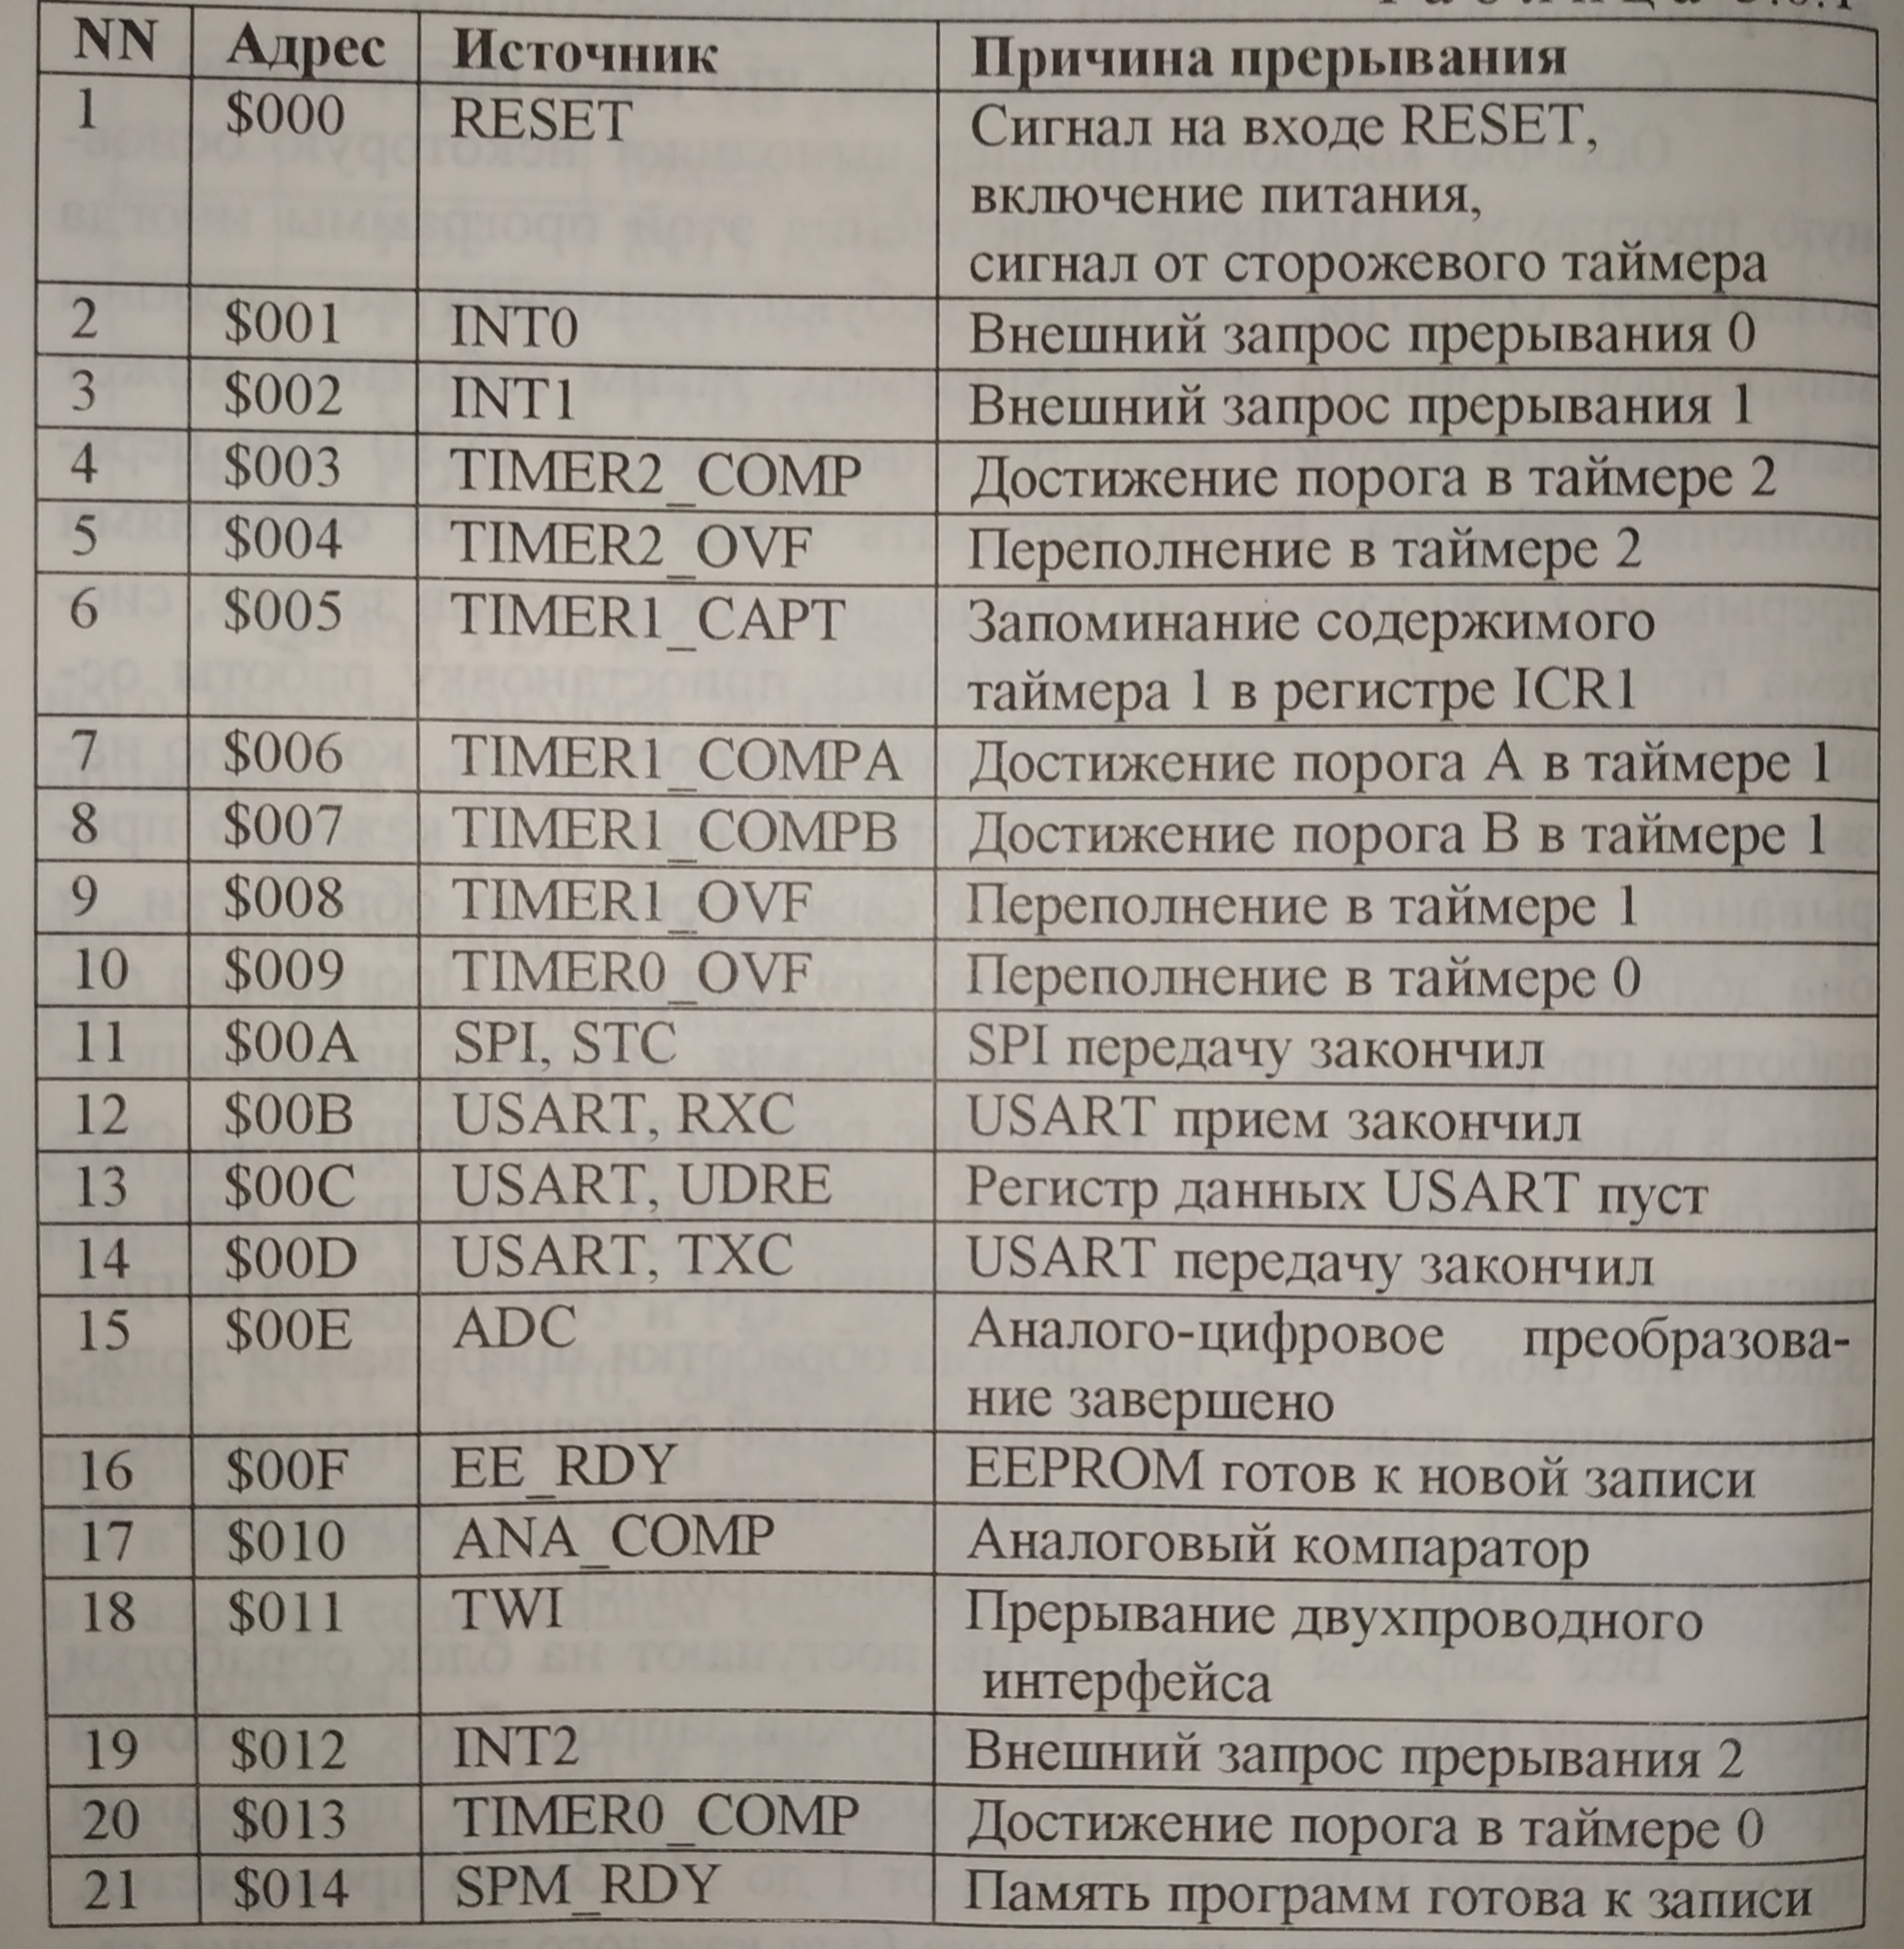
\includegraphics[width=0.5\linewidth]{pics/27.jpg}
  }
  \caption{Таблица прерываний.}
  \label{img::table}
\end{figure}

На рис. \ref{img::table} представлена таблица прерываний. При выполнении некой программы иногда возникают события или запросы прерывания (нажатие кнопки
$INT0$ или переполнение таймера). В результате чего система прерываний должна остановить
работу основной программы и запустить программу обработки прерываний. Для каждого действия 
своя. Все запросы поступают на блок обработки (Interrupt Unit), который определяет номер 
запроса ($1-21$) и возможность выполнения. В случае разрешенного прерывания чувствительность
ко всем прерываниям запрещается (в $7$-й разряд регистра флагов записывается $0$). Текущее 
содержимое записывается в стек, на его место заносится адрес прерывания из таблицы векторов 
прерываний. Если необходимо несколько прерываний, то они будут выполнены в порядке приоритета 
от наименьшего номера.

$RJMP$ -- команда к началу прерывания (относится к командам безусловной передачи управления)

$NOP$ -- нет операции



\section{Сколько всего прерываний у ATmega8535.}
Всего $21$ прерывание. Среди них $4$ -- внешние 
и вызываются сигналами, приходящими на выводы микроконтроллера
$INT0$, $INT1$, $INT2$, $RESET$. Остальные $17$ -- внутренние, обслуживают
дополнительные блоки.


\section{Как организовать вложенные прерывания.}
Вложенные прерывания становятся возможными в начале программы обработки
прерывания, тогда можно осуществить разрешение прерываний. Однако 
возможно переполнение стека ($512$ байт) при большом уровне вложенности.


\section{Как можно разрешить (запретить) одновременно все прерывания.}
Прерывания не будут обрабатываться если в разряде $7$ регистра флагов 
стоит $0$ (общее запрещение прерываний). Осуществляется командами:
\begin{verbatim}
  sei ; разрешить прерывания
  cli ; запретить прерывания
\end{verbatim}

\section{Как организована система приоритетов при обработке прерываний. }
Если одновременно возникает несколько прерываний, то первым будет 
обрабатываться прерывание, имеющее наименьший номер в таблице прерываний, представленной на рис. \ref{img::table}

\section{Какое минимальное время требуется для преобразования в АЦП.}
Минимальное время преобразования аналого-цифрового преобразователя 
составляет $65$ микросекунд.

\section{Чем сигнальный процессор отличается от МК.}

Сигнальный процессор обеспечивает обработку информации, выполняя команды в соответствии с 
системой команд микроконтроллера. 
МК – интегральная схема, которая может принимать сигналы от датчиков, обрабатывать и 
выдавать управляющие сигналы на исполнительные механизмы для выполнения поставленной задачи 
(работает с периферией).

\section{Зачем в программе надо устанавливать начальное значение Stack Pointer и чему это значение должно быть равно.}

Указатель стека $SP$ (Stack Pointer) предназначен для работы со стеком, имеет $10$ разрядов, 
состоит из $2$-х $8$-разрядных регистров ($SPH$-старший байт, $SPL$-младший байт). Обращение 
через команды $IN$, $OUT$. После команды $RESET$ значение $0$. 
Текущее содержимое $SP$ определяет положение вершины стека. 

\section{Сторожевой таймер и особенности его работы.}

WatchDog Timer – предназначен для ликвидации сбоев в работе МК, возникающих из-за различного
рода помех. $WDT$ через определенный заданный промежуток времени вырабатывает сигнал сброса 
($RESET$) МК, перезапуская рабочую программу. Для обнаружения сбоев и предотвращения 
перезапуска при правильной работе в нее включают команду $WDR$ (Watch Dog Reset) 
осуществляющей сброс сторожевого таймера, в результате отсчет времени начинается заново.

\section{Что такое SPI и зачем он нужен.}

Последовательный синхронный интерфейс SPI - serial peripheral interface или интерфейс связи
устройств, позволяет передавать данные с высокой скоростью между МК и внешними устройствами.
Свойства:
\begin{enumerate}
  \item Полнодуплексная (одновременно в $2$-х направлениях) $3$-х проводная синхронная
        передача данных. 
  \item Предельная скорость передачи данных СК/$4$ бит/сек 
  \item Передача осуществляется байтами.
  \item Передавать можно старшим либо младшим битом вперед  
  \item По окончании вырабатывается прерывание (адрес $\$008$) 
  \item Имеется флаг конфликтов при записи $WCOL$ (Write Collision Flag) 
\end{enumerate}	

\section{Как инициировать передачу байта в SPI.}

Для нормального подключения необходимо:
\begin{itemize}
  \item Для MASTER настроить MOSI, SCL, SS на выход, MISO на вход.
  \item Для SLAVE настроить MOSI, SCL, SS на выход, MISO на выход.
  \item При соединении одноименные выводы подключаются друг к другу, выставив $SS$ на ведомом 
        устройстве в $0$. 
\end{itemize}

\section{Сколько прерываний и сколько регистров ввода/вывода принадлежит SPI.}

Одно прерывание: SPIE – Interrupt Enable. Разрешение прерывания после передачи байта. 
(SPE – SPI Enable. Разрешение работы SPI. Если в этом разряде $0$, то никакие функции SPI 
не будут реализованы)

3 регистра: 
\begin{enumerate}
  \item SPI STATUS REGISTER (SPSR) - контрольный, можно использовать только для чтения,
        после RESET все $0$. 
  \item SPI CONTROL REGISTER (SPCR) - состояния - можно использовать для чтения и записи,
        после RESET все $0$.
  \item SPI Data Register (SPDR) - под данные - можно использовать для чтения и записи,
        после RESET все $0$. 
\end{enumerate}

\section{Далее пойдут вопросы про однопроводный интерфейс (сеть MicroLAN).}

Ждёмс

\section{Сколько проводов необходимо для реализации однопроводного интерфейса.}

Для уменьшения количества физических соединений в микропроцессорных системах энергонезависимая
память, устройства контроля доступа, датчики температуры, цифровые переключатели, мониторы
аккумуляторных батарей и многие другие узлы часто подключаются с помощью всего двух проводов,
используемых как для питания, так и передачи информации. Поскольку один из проводов является
общим, то такой способ подключения стал называться однопроводным.

\section{Как выглядит физический ноль и физическая единица.}

Физический ноль -- низкое напряжение, физическая единица -- высокое.

\section{Как в однопроводном интерфейсе передается информационный ноль и информационная единица? Какова максимальная скорость  передачи?}

В однопроводном интерфейсе передаются информационный ноль и информационная единица -- 
логически; максимальная скорость  передачи $0$ -- длинный импульс физического нуля ($60$ мкс),
$1$ - короткий ($15$ мкс).

\section{Что такое серийный номер в однопроводном интерфейсе и какова его структура.}

Серийный номер в однопроводном интерфейсе -- $64$ бита: $8$ бит -- код семейства, $48$ бит -- 
серийный номер, $8$ бит -- контрольная сумма - уникальный идентификатор устройства, 
чтобы можно было выбрать устройство.

\section{Какая команда позволяет Master определить номера всех Slave в сети MicroLAN.}

Search ROM

\section{Как выглядит сигнал сброса в сети MicroLAN.}

Сигнал сброса в сети MicroLAN: Долгий импульс нуля ($480$ мкс), потом долгий импульс единицы, 
в течении которой master проверяет, есть ли кто-нибудь в сети.
